\documentclass[•]{article}
\usepackage{graphicx, float}
\usepackage{caption}
\usepackage{subcaption}
\usepackage{verbatim}
\author{Tijmen Wintjes}
\title{Support Vector Classification \\ Session 2}

%%
\begin{comment}
\begin{figure}[h!]
\centering
\begin{minipage}{.45\textwidth}
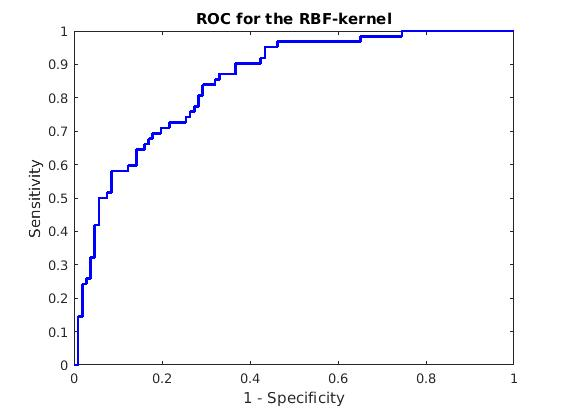
\includegraphics[width=.8\textwidth]{rocrbfdiabetes.jpg}
\end{minipage}
\begin{minipage}{.45\textwidth}
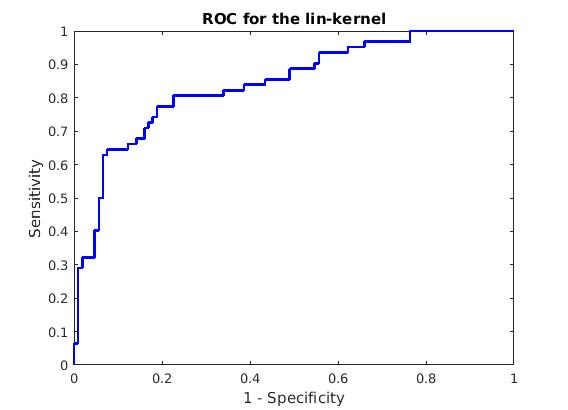
\includegraphics[width=.8\textwidth]{roclindiabetes.jpg}
\end{minipage}
\caption{ROC-curve of a RBF-classifier and a linear classifier on the diabetes data-set.}
\end{figure}
\end{comment}
%%

\newcommand{\apicture}[2] {
  \begin{figure}[H]
  \centering
  \includegraphics[width=0.5\textwidth]{#1}
  \caption{#2}
  \end{figure}
}

\begin{document}
\maketitle
\section{Function Estimation}
\subsection{Support Vector Machine for regression}
The twenty data-points I created are displayed below.

\apicture{datagen.png}{The data generated for the 'uiregress' function.}

All kernels available in 'uiregress' funciton of the SVM-toolbox were applied. The results for the linear, linear spline and rbf-kernel are displayed below. The RBF-kernel performs best.

\begin{figure}[H]
\centering
\begin{minipage}{.3\textwidth}
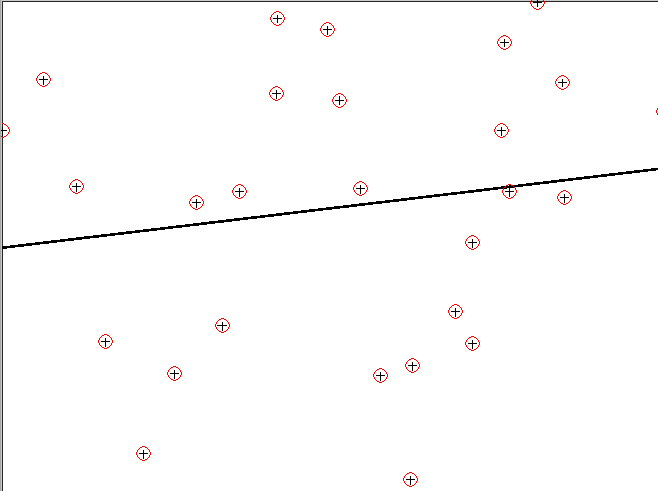
\includegraphics[width=.8\textwidth]{estlin.png}
\end{minipage}
\begin{minipage}{.3\textwidth}
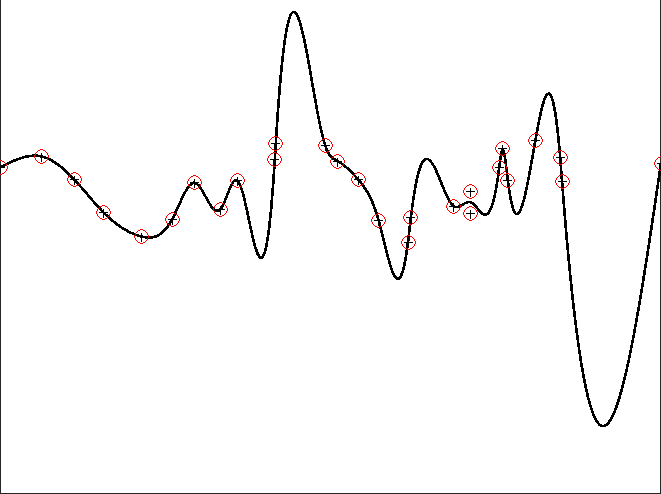
\includegraphics[width=.8\textwidth]{estlinspline.png}
\end{minipage}
\begin{minipage}{.3\textwidth}
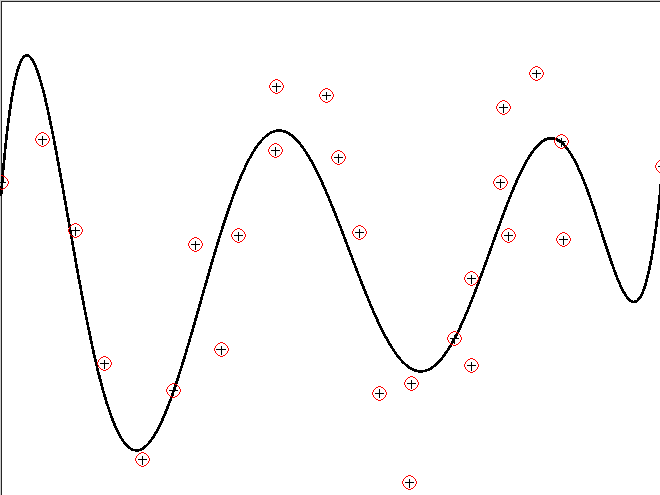
\includegraphics[width=.8\textwidth]{estrbf.png}
\end{minipage}
\caption{Estimations of the trigonometric function with various kernels.}
\end{figure}

Next we investigate the effect of the hyperparameter $e$. It gives the band around the estimated function for which data points lying inside have been estimated perfectly. Increasing it makes the estimation less sensitive to noise, but also less precise. 

\begin{figure}[H]
\centering
\begin{minipage}{.3\textwidth}
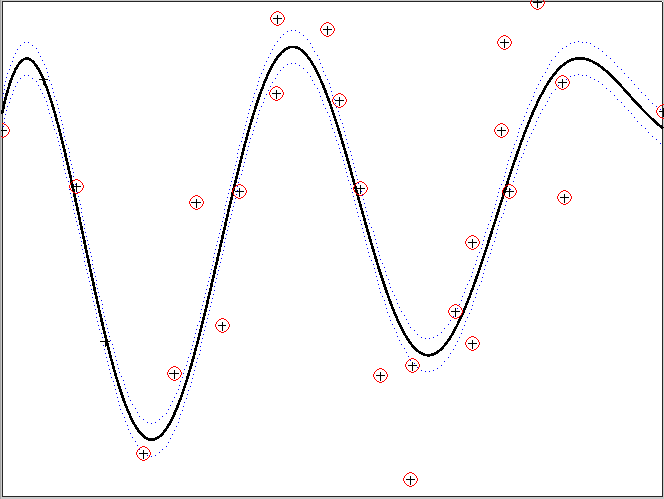
\includegraphics[width=.8\textwidth]{e01.png}
\end{minipage}
\begin{minipage}{.3\textwidth}
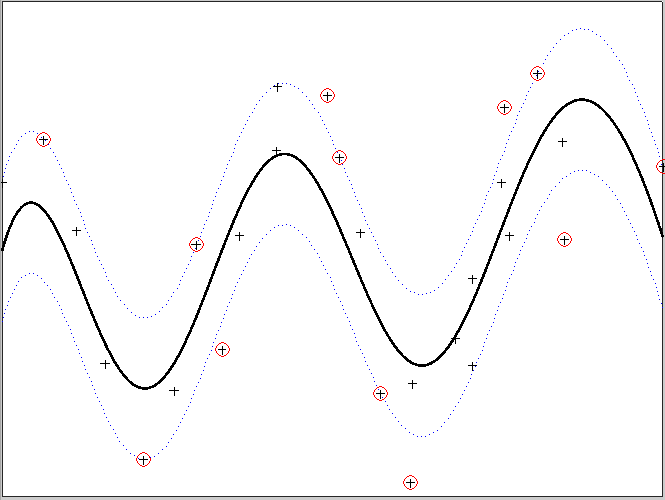
\includegraphics[width=.8\textwidth]{e25.png}
\end{minipage}
\begin{minipage}{.3\textwidth}
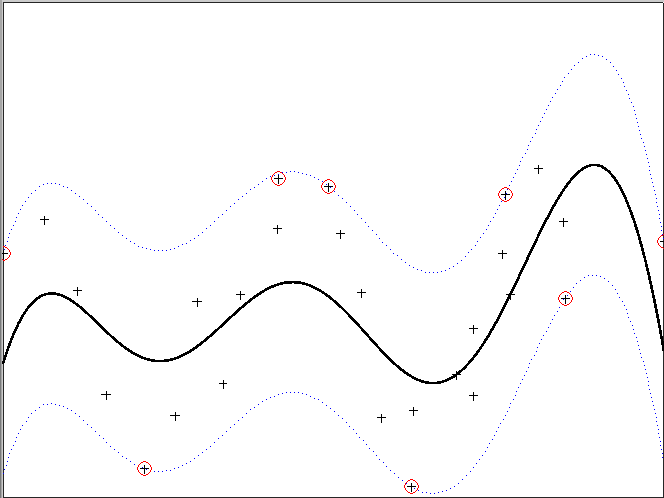
\includegraphics[width=.8\textwidth]{e1.png}
\end{minipage}
\caption{The effect of the hyperparameter $e$, from left to right $e=0.01$, $e=0.05$ and $e=0.1$. $\sigma = 2$.}
\end{figure}

The bound parameter defines the penalty on misclassification. If this value is very low. The estimation is not sensitive enough. Setting it too high makes the estimation sensitive to outliers.

\begin{figure}[H]
\centering
\begin{minipage}{.3\textwidth}
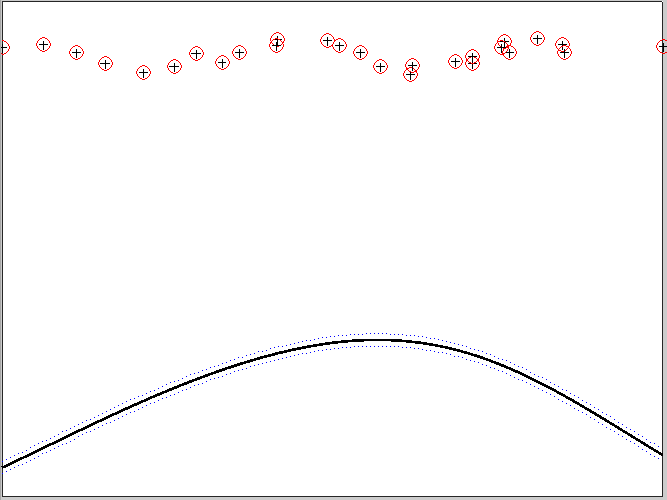
\includegraphics[width=.8\textwidth]{bound01.png}
\end{minipage}
\begin{minipage}{.3\textwidth}
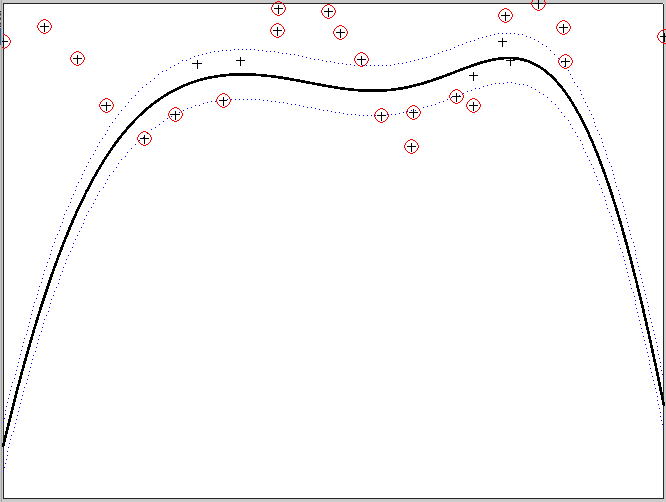
\includegraphics[width=.8\textwidth]{bound1.png}
\end{minipage}
\begin{minipage}{.3\textwidth}
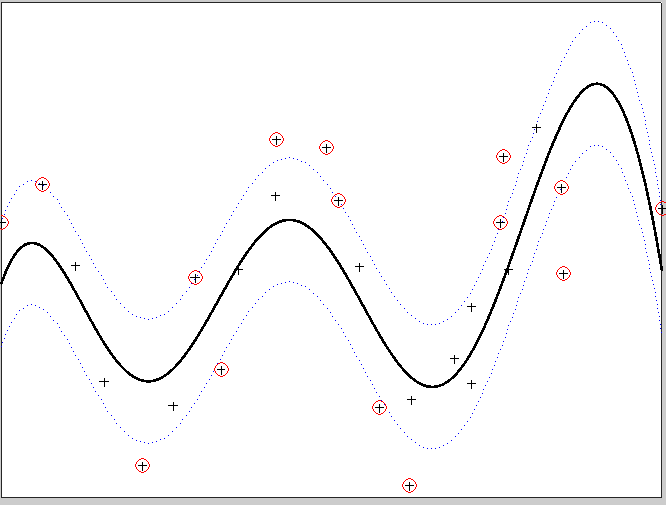
\includegraphics[width=.8\textwidth]{bound10.png}
\end{minipage}
\caption{The effect of the hyperparameter $Bound$, from left to right $Bound=0.1$, $Bound=1$ and $Bound=10$. $\sigma = 2$.}
\end{figure}

In figure 3 we can nicely see that increasing $e$ leads to sparsity of the vector with support vector values. SVM is different form least-square function estimation in the metric it uses to minimize. As long as points are within the $e$-band they are treated as if they lie exactly on the line itself and their distance has cost = 0. 

\subsection{A simple example: The $sinc$}
For a first exploration of the function estimation abilities of the lssvm we use a noisy sinc function. 

\apicture{noisysinc.jpg}{Plot of the noisy sinc function}

\begin{figure}[H]
\centering
\begin{minipage}{.45\textwidth}
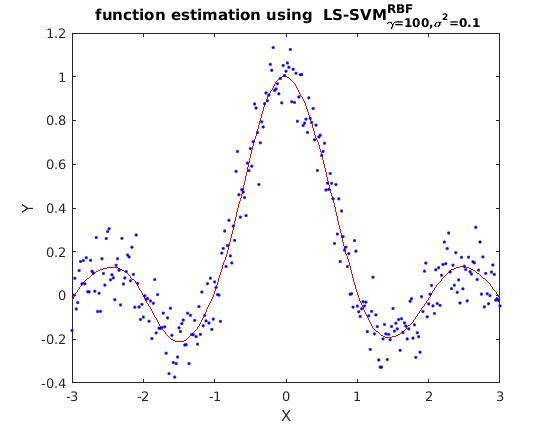
\includegraphics[width=.8\textwidth]{rbfestsinc.jpg}
\end{minipage}
\begin{minipage}{.45\textwidth}
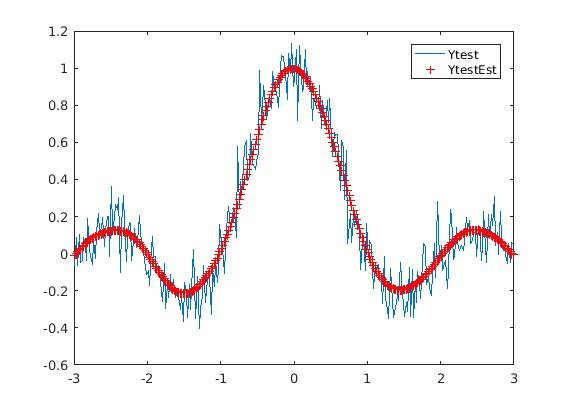
\includegraphics[width=.8\textwidth]{rbfesttest.jpg}
\end{minipage}
\caption{On the left a plot of the estimated function using an lssvm with rbf-kernel, $\sigma = 1$ and $\gamma= 100$, on the right a comparison with the test data.}
\end{figure}

\subsection{Hyper-parameter tuning}
Tuning of the hyper-parameters $\sigma$ and $\gamma$ was carried out with both a gridsearch and simplex optimization scheme. The difference between the two being that gridsearch is a brutforce method, while simplex uses an algorithm devised by Nedler and Mead to iteratively find values of $\sigma$ and $\gamma$ which lead to lower costs. The optima found are however not unique, rerunning 'tunelssvm' multiple times leads to different results. However the final value of the objective function stays level with respect to the sought accuracy. Qualitatively there seems to be little difference between the two methods. 

\begin{figure}[H]
\centering
\begin{minipage}{.45\textwidth}
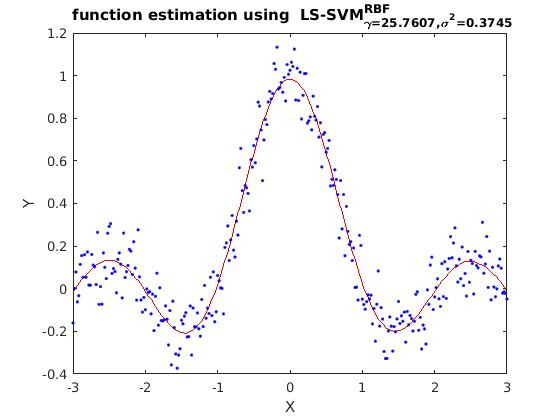
\includegraphics[width=.8\textwidth]{rbfestgrid.jpg}
\end{minipage}
\begin{minipage}{.45\textwidth}
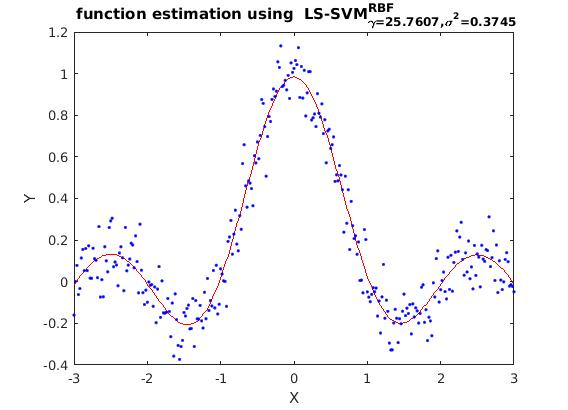
\includegraphics[width=.8\textwidth]{rbfestsimplex.jpg}
\end{minipage}
\caption{On the left a plot of the estimated function using 'gridsearch' to find  $\sigma$ and $\gamma$, on the right we used 'simplex'}
\end{figure}

\subsection{Application of the Bayesian Framework}
Another way to tune hyper-parameters is by using the bayesian interference framework for a lssvm. Page 120 of the course notes gives a decent graphical overview of how conceptually the levels of interference are related. Interference for the function estimation problem of the sinc function leads to the following result.

\apicture{bayesianest.jpg}{Plot of the lssvm with hyper-parameters infered by the bayesian framework}

Bayesian inference also allows us to define a posterior class probability in classification problems. For the iris data set such a approach was taken in the figure below. The figures show that choices of the hyper-parameters that are not optimal result in a blurring of the decision boundary. Left a picture of the posterior class probability for the $\gamma = 0.5$ and $\sigma = 0.75$, the left two pictures are made with in the middle $\gamma = 10$ and on the right $\sigma = 10$.  The colors give us the probability that a data point within that area belongs to a class.


\begin{figure}[H]
\centering
\begin{minipage}{.3\textwidth}
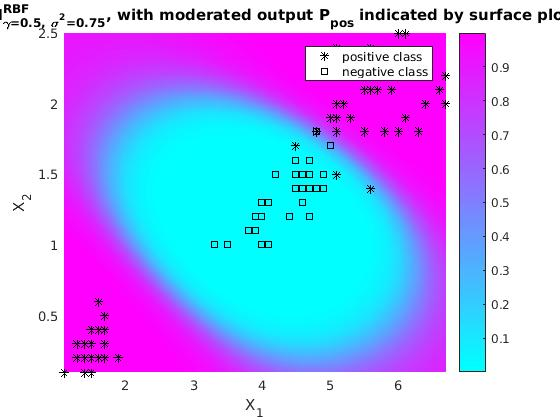
\includegraphics[width=.8\textwidth]{irisclassprob.jpg}
\end{minipage}
\begin{minipage}{.3\textwidth}
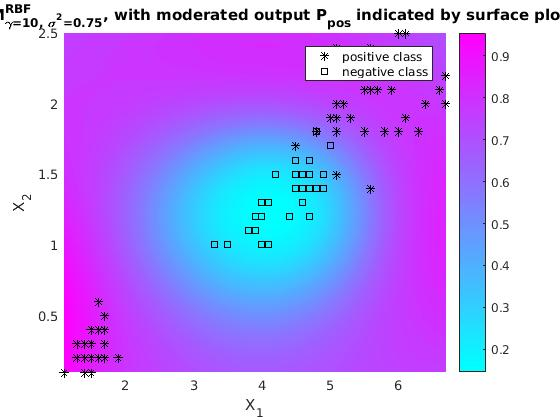
\includegraphics[width=.8\textwidth]{gammablur.jpg}
\end{minipage}
\begin{minipage}{.3\textwidth}
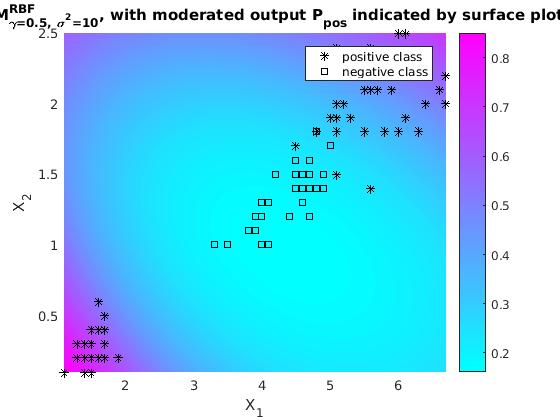
\includegraphics[width=.8\textwidth]{sigmablur.jpg}
\end{minipage}
\caption{The effect of the hyperparameter $\gamma$ and $\sigma$ on the decission boundary of the iris data-set.}
\end{figure}

The bayesian network can also be used for Automatic Relevance Detection, which means trying to to couple an output to inputs which in some metric seems to be best corresponding. Coupling the randomized input of the sinc to output we get the following figures:

\begin{figure}[H]
\centering
\begin{minipage}{.3\textwidth}
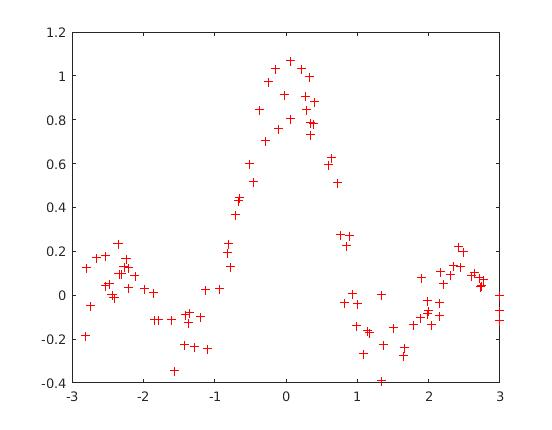
\includegraphics[width=.8\textwidth]{inout1.jpg}
\end{minipage}
\begin{minipage}{.3\textwidth}
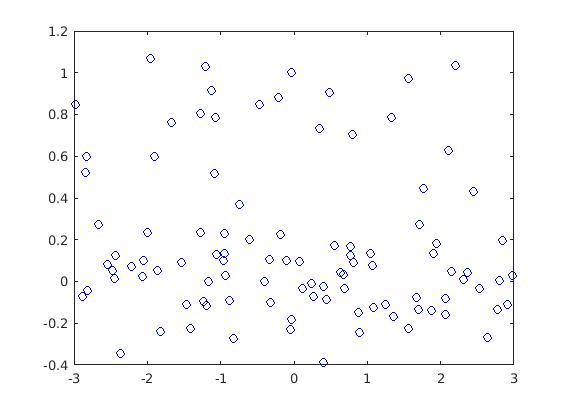
\includegraphics[width=.8\textwidth]{inout2.jpg}
\end{minipage}
\begin{minipage}{.3\textwidth}
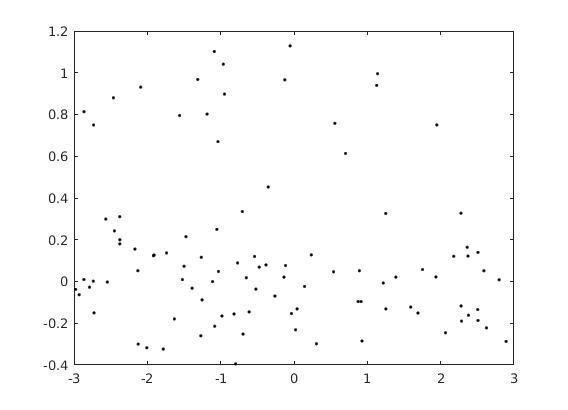
\includegraphics[width=.8\textwidth]{inout3.jpg}
\end{minipage}
\caption{Three different randomized x-value inputs and the corresponding sinc output for one of them.}
\end{figure}

The bayesian ARD function suggest that the first input is probably the input that generated the data. A similair result can be obtained by performing crossvalidation with an RBF-kernel. For the different plots we sort the cost returned by the crossvalidation and rank them from low to high cost. This will be the corresponding ranking.

\subsection{Robustness}
This subsection discusses the robust methods of the lssvm toolbox. Adding a couple of outlier to the noisy sinc function and estimating it a normal way makes clear that outliers have a big effect on the least square method. 

\apicture{noisysincout.jpg}{Plot of the estimated noisy sinc with outliers}

For the robust case we prefer the mean absolute error over the mean squared error. The squared error amplifies the cost of having data points far away from the estimated curve, which in this case we don't mind, therefore we take the mean absolute error which is less sensitive. Page 152/153 give a clear overview. We fit the sinc function with four different loss functions. The huber and logistic function have a ceiling for the cost of the strong outliers, but still count the. The Hampel and Myriad function barely take them into consideration at all.

\begin{figure}[H]
\centering
\begin{minipage}{.45\textwidth}
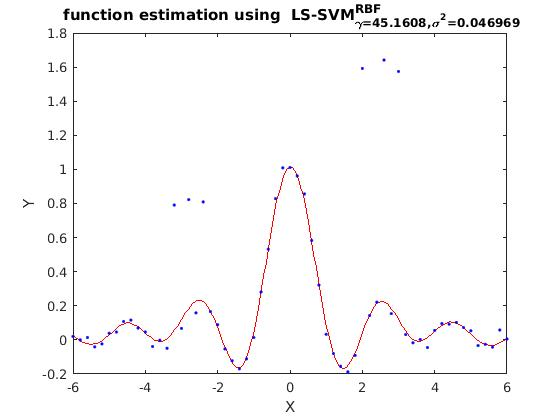
\includegraphics[width=.8\textwidth]{robusthuber.jpg}
\end{minipage}
\begin{minipage}{.45\textwidth}
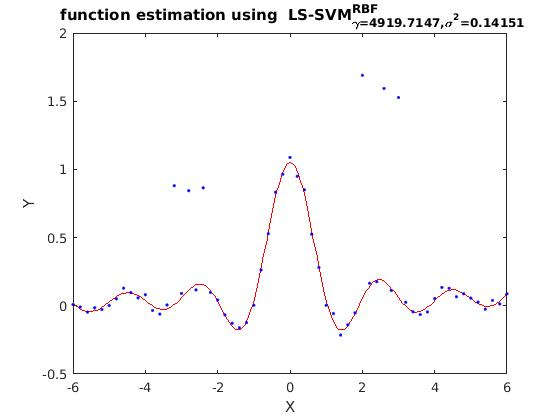
\includegraphics[width=.8\textwidth]{robusthampel.jpg}
\end{minipage}
\begin{minipage}{.45\textwidth}
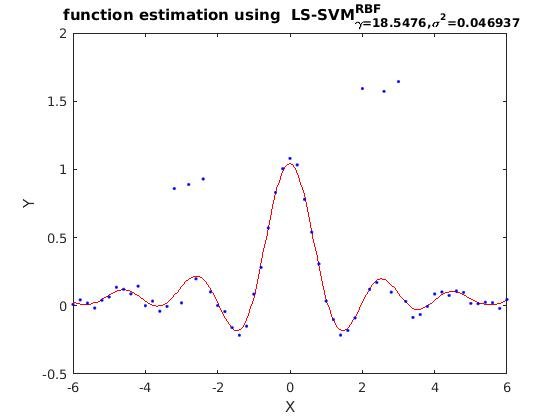
\includegraphics[width=.8\textwidth]{robustlogistic.jpg}
\end{minipage}
\begin{minipage}{.45\textwidth}
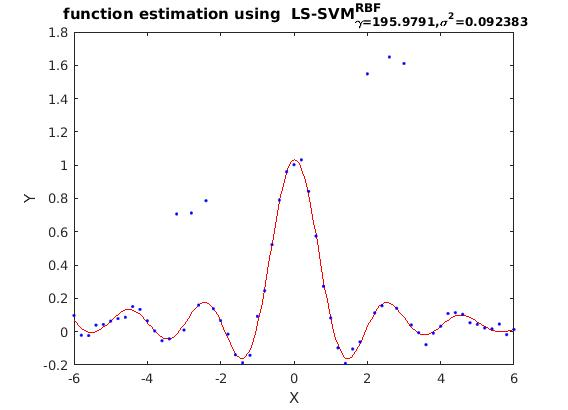
\includegraphics[width=.8\textwidth]{robustmyriad.jpg}
\end{minipage}
\caption{Four different robust estimations with differnt cost function. Top left Huber, top right hampel, bottom left logistic, bottom right myriad.}
\end{figure}

\section{Homework}
The NAR model was estimated on the full data-set leading to the following result:
\apicture{ARmodel.jpg}{Output of plotlssvm with order = 10.}

To estimate an appropiate order we tuned the parameters $\sigma$ and $\gamma$ for every order between 5 and 25. With the crossvalidation function we checked how the model of a certain order performed. Leading to the following graph:

\apicture{paramplot.jpg}{Plot of the cost as given by crossvalidation for different orders.}

This leads to the decision to keep an order of 10. Testing on the testset gives the following result. Increasing the order leads to bad results on the testset due to overfitting.

\begin{figure}[H]
\centering
\begin{minipage}{.3\textwidth}
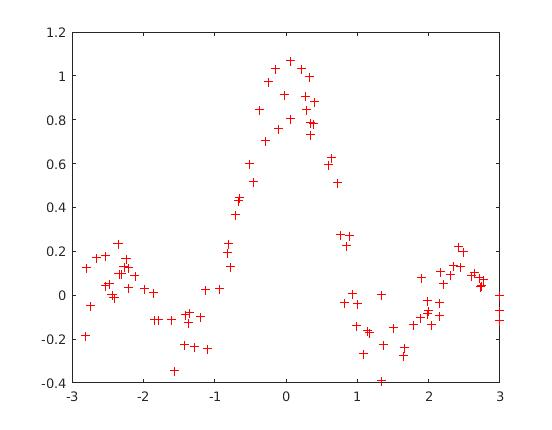
\includegraphics[width=.8\textwidth]{inout1.jpg}
\end{minipage}
\begin{minipage}{.3\textwidth}
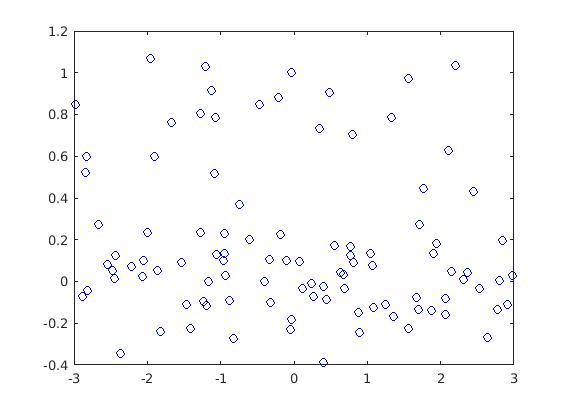
\includegraphics[width=.8\textwidth]{inout2.jpg}
\end{minipage}
\begin{minipage}{.3\textwidth}
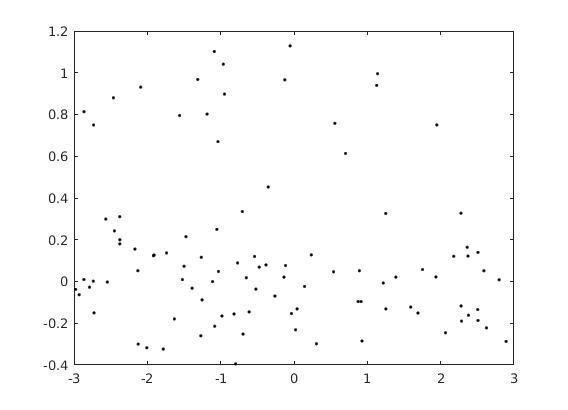
\includegraphics[width=.8\textwidth]{inout3.jpg}
\end{minipage}
\caption{Three plot of predicted values of the NAR model with order = 10, 15 and 20.}
\end{figure}


\end{document}